\section{Compilation}
\label{sec:compilation}

The front-end language of \sysname is designed to simplify operators' task of describing preferred paths. That simplicity, however, comes at the cost of compilation complexity. The compiler must efficiently compute the sets of paths represented by the intersection of preferences and topology, compute which ones can be honored under a given failure scenario, and ensure policy compliance under all possible failure cases. We handle this challenge by breaking down the compilation task into multiple stages and developing efficient algorithms for each.

\subsection{Overview}

\begin{figure}[t!]
\centering
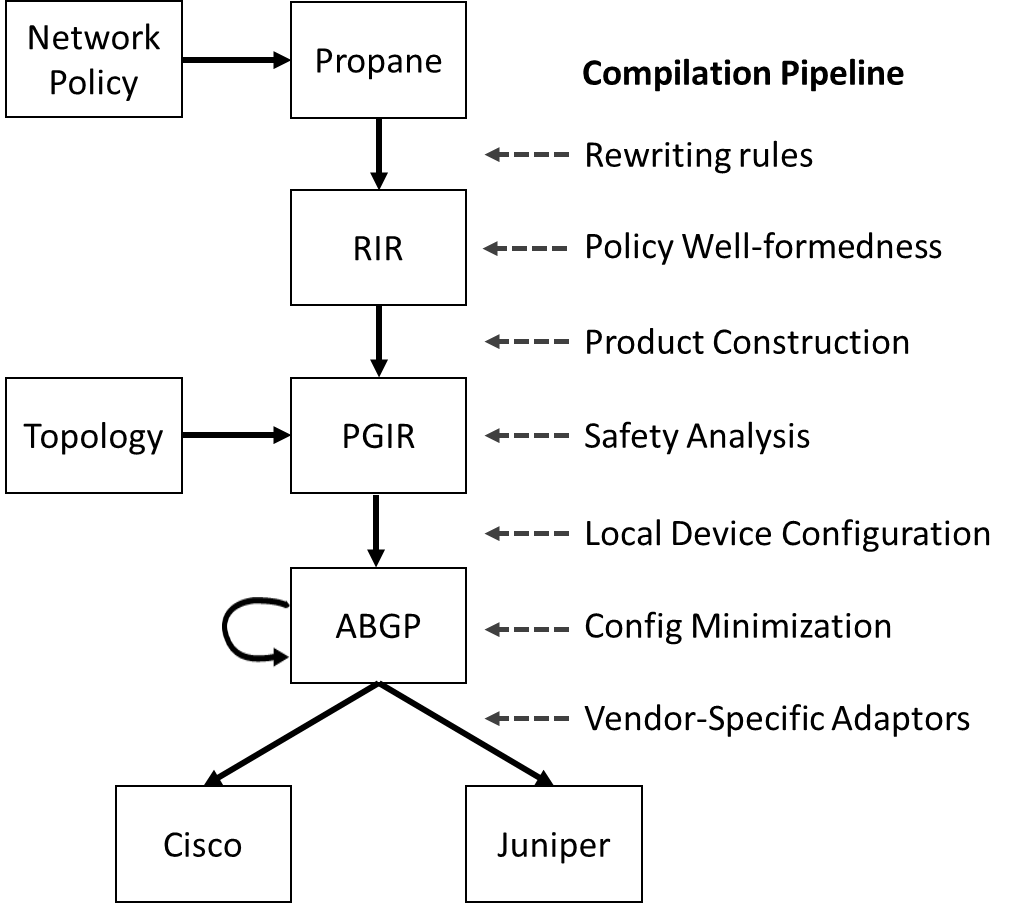
\includegraphics[width=\columnwidth]{figures/pipeline}
\caption{Compilation pipeline stages for Propane.}
\label{fig:pipeline}
\end{figure}

%In this section we briefly describe our compilation strategy for \sysname. 

Figure~\ref{fig:pipeline} shows the 5 stage compilation pipeline to translate user-level \sysname policies into device-local BGP policies. The first stage of the pipeline involves simple rewriting rules and substitutions from the user-level language into the core Regular Intermediate Representation (RIR). Policies in RIR are checked for well-formedness (e.g., never constraining traffic that does not enter the network), before being combined with topological information to obtain the Product Graph Intermediate Representation (PGIR). The PGIR is a data representation that compactly captures the control flow of all BGP advertisements subject to the policy and topology restrictions. We develop efficient algorithms that operate over the PGIR to ensure policy compliance under failures, avoid BGP instability, and prevent aggregation-induced black holes. Once the compiler determines the PGIR for the policy is safe, it uses a simple translation to an abstract BGP (ABGP) representation. To make configurations more readable for human operators, and to reduce the size of the resulting configurations, the \sysname compiler makes several passes over the ABGP form. Finally, vendor-specific adaptors can be added to \sysname to translate from ABGP to actual concrete configurations that go on the network devices.


\subsection{Regular IR (RIR)}
\label{sec:rir}

The high-level language of \S\ref{sec:propane} is just a thin layer on top of a core, regular-expression-based language for describing preference-based path constraints. Regular expressions are an expressive formalism that have been studied extensively for their utility in describing paths through graphs~\cite{bib:todo}, with applications to networks~\cite{bib:todo}. Our regular expression language differs from others by allowing operators to describe preferences between paths.

% grammar
\newcommand{\BNFALT}{\;\;|\;\;}
\newcommand{\hdr}[2]{\flushleft \chdr{#1}{#2}}
\newcommand{\chdr}[2]{\textbf{#1} {#2} \\ \centering}

\begin{figure*}
  \begin{minipage}[t]{.45\linewidth}
  \hdr{\large Syntax}{}
  \vspace*{-1\baselineskip}
  %
  \[ \begin{array}{rclr}
    \hline

     pol     &::=& p_1, \dots, p_n & \textit{constraints} \\
     p       &::=& t \mapsto r_1 \gg \dots \gg r_m & \textit{preferences} \\
     t       &::=& & \textit{test} \\
         &\BNFALT& true & \textit{true} \\
         &\BNFALT& \neg t & \textit{negation} \\
         &\BNFALT& t_1 \vee t_2 & \textit{disjunction} \\
         &\BNFALT& t_1 \wedge t_2 & \textit{conjunction} \\
         &\BNFALT& prefix = x & \textit{prefix test} \\
         &\BNFALT& comm = c & \textit{community test} \\
     r       &::=& & \textit{regular paths} \\
         &\BNFALT& n & \textit{AS number} \\
         &\BNFALT& in & \textit{internal loc} \\
         &\BNFALT& out & \textit{external loc} \\
         &\BNFALT& r_1 \cup r_2 & \textit{union} \\
         &\BNFALT& r_1 \cap r_2 & \textit{intersection} \\
         &\BNFALT& r_1 \cdot r_2 & \textit{concatenation} \\
         &\BNFALT& !(r) & \textit{path negation} \\
         &\BNFALT& r^* & \textit{repetition} \\
     l       &::=& r_1 \rightarrow r_2 & \textit{link pairs} \\
     cc     &::=& agg(x, l) \BNFALT tag(c, t, l) & \textit{control constraints} \\
  \end{array} \]

  \end{minipage}
  %
  ~~
  \vrule
  ~~
  %
  \begin{minipage}[t]{.5\linewidth}
  \hdr{\large Propane Expansions}{}
  \vspace*{-1\baselineskip}
  %
  \[ \begin{array}{rcl}
    \hline
    any           & = & out^* \cdot in^+ \cdot out^* \\
    internal      & = & in^+ \\
    external      & = & out^+ \\
    only(X)       & = & any \cap X^* \\
    never(X)      & = & any \cap (!X)^* \\
    through(X)    & = & out^* \cdot in^* \cdot X \cdot in^* \cdot out^* \\
    after(X)      & = & out^* \cdot (X \cap out) \cdot out^* \cdot in^+ \cdot out^* \\
    before(X)     & = & out^* \cdot in^+ \cdot out^* \cdot (X \cap out) \cdot out^* \\
    end(X)        & = & any \cap (\Sigma^* \cdot X) \\
    start(X)      & = & any \cap (X \cdot \Sigma^*) \\
    exit(X)       & = & (out^* \cdot in^* \cdot (X \cap in) \cdot out \cdot out^*) \cup \\
                  &        & (out^* \cdot in^+ \cdot (X \cap out) \cdot out^*) \\
    enter(X)      & = & (out^* \cdot out \cdot (X \cap in) \cdot in^* \cdot out^*) \cup \\
                  &        & (out^* \cdot (X \cap out) \cdot in^+ \cdot out^*) \\
    link(X,Y)     & = & any \cap (\Sigma^* \cdot X \cdot Y \cdot \Sigma^*) \\
    path(\vec{X}) & = & any \cap (\Sigma^* \cdot X_1 \dots X_n \cdot \Sigma^*) \\
    novalley(\vec{X}) & = & any ~ \cap \\
                  &   & !path(X_2,X_1,X_2) ~ \cap \dots \cap \\
                  &   & !path(X_n,X_{n-1},X_n) \\
  \end{array} \]

  \end{minipage}

  \hrulefill

  \caption{Regular Intermediate Language (RIL) syntax (left), and
           Propane language expansions (right).}
  \label{fig:rir-syntax}
\end{figure*}


\para{Syntax}

The syntax for the RIR is shown in Figure~\ref{fig:rir-syntax}. A policy consists of one or more constraints, each of which consists of a test on the type of route, and a corresponding set of preferred regular paths. Regular paths are simply regular expressions where the base characters are abstract locations - either a router or an Autonomous System (AS) number. Special \textit{in} and \textit{out} symbols are used to refer to any internal or external location respectively.
For example, the constraint
$$prefix=74.125.28.0/24 \mapsto (AS200 \cdot in^+) \gg (AS100 \cdot in^+)$$
describes a more-preferred set of paths for traffic announced by a prefixes no less specific than $74.125.28.0/24$, which starts at AS 200, before entering and staying inside the user's network to get to the destination, and a less-preferred set of paths that start at AS 100 and are otherwise the same. The plus operator $in^+$ stands for $in \cdot in^*$ in the usual way. Tests over route types use standard boolean connectives, and can refer to both prefixes and route community values.

\sysname also supports constraints purely on the control-plane behavior of the BGP routing protocol. Thing like prefix aggregation, which should not affect routing behavior, is an important optimization to reduce routing table size and churn in practice. Aggregation, for example from internal locations and external locations, is specified using the same regular syntax as before:
$$agg(128.17.0.0/16, in \rightarrow out)$$
where the expression $in \rightarrow out$ refers to control messages flowing from any internal location to any external location.

We list the route aggregation and community tagging constraints in Figure~\ref{fig:rir-syntax}, however our implementation also supports other constraints such as limiting the maximum number of routes allowed between ASes, or enabling BGP multipath.


\para{Semantics}

The semantics of RIR can be thought of in terms of ranked paths. Each preference-based regular path constraint (of the form $r_1 \gg \dots \gg r_j$) maps to a set of concrete paths in the network that match one of $r_i$. We denote a network path as a string of abstraction locations (routers or external ASes) of the form: $n_1 n_2 \dots n_k$, and we say regular expression $r$ matches path $p$, if $p \in \mathcal{L}(r)$ and $p$ is a topologically-valid path. We denote the length of a path $p$ as $\abs{p}$. A path $p$ will have a rank:
$$(\min_i \set{ p \in \mathcal{L}(r_i) }, \abs{p})$$
where the rank is lexicographically ordered according to (1) the most preferred regular expression matched, and (2) as a tie breaker, the length of the path. A lower rank indicates a \emph{more} preferred path. The desired semantics is to allow traffic to be sent along any of the most preferred paths for each pair of starting and ending locations that appear in some valid specified path.

The set of ranked paths depends on which paths are valid given the topology, and thus when failures occur, so do the most preferred routes. It is the job of the \sysname compiler to ensure that generated configurations for a policy always achieve the most preferred path possible given the failures in the topology, using only distributed mechanisms.


\para{Propane front-end to RIR}

The main differences between the \sysname front-end language and the RIR are: (1) \sysname allows the programmer to specify constraints separately, and combine them together modularly, (2) \sysname provides high-level names that abstract sets of routes, and (3) \sysname allows the preference operator to be used locally.

One of the main constraints when translating to RIR is to ensure that all specified routes are well-formed. In particular, each regular path constraint $r$ must satisfy $r \subseteq out^* \cdot in^+ \cdot out^*$. This ensures that one can only ever talk about controlling traffic that goes through the user's network at some point.

The translation from \sysname to RIR is based on a set of simple rewriting rules.
The first step is to merge separate constraints. This is accomplished by simply taking the cross product of per-prefix constraints, where logical conjunction ($a \wedge b$) is replaced by intersection on regular constraints ($a \cap b$), logical disjunction is replaced by union, and logical negation ($\neg a$) is replaced by ($any \cap !(a)$), where $any$ ensures the routes are well-formed.
%
For example, in the data center configuration from Section~\ref{sec:propane}, combining the \textit{Routing} and \textit{Ownership} constraints would result in the following RIR configuration:

\begin{lstlisting}[mathescape=true]
$\path{p_{g1}}{any \cap end(A)}$
$\path{p_{g2}}{any \cap end(B)}$
$\path{p_{l1}}{\neg enter(out) \cap end(E)}$
$\path{p_{l2}}{\neg enter(out) \cap end(F)}$
$\path{true}{exit(out)}$
\end{lstlisting}

The next step is to rewrite the high-level constraints such as \textit{enter} and \textit{exit} according to the equivalences listed in Figure~\ref{fig:rir-syntax}. Since preferences can only occur at the outermost level for an RIR expression, the final step is to lift occurences of the preference operator that occur in the regular expression. For example, the regular expression $a \cdot (b \gg c) \cdot d$ is lifted to $(a \cdot b \cdot d) \gg (a \cdot c \cdot d)$ by distributing the preference over the sequence operator. In general, we employ the follwing equivalence:
%
$$x \odot (y_1 \gg \dots \gg y_n) = x \odot y_1 \gg \dots \gg x \odot y_n$$
%
where $\odot$ stands for an arbitrary regular binary operator. Preferences nested under a unary operator, \textit{star} or \textit{negation}, are flagged by the compiler as invalid policies.



\subsection{Product Graph IR}


\newcommand{\state}[4]{\node[state,#3](#1)[#4]{#2};}
\newcommand{\transition}[4]{\path[->] (#1) edge [#4] node {#3} (#2);}


\begin{figure*}
  \begin{minipage}[t]{.5\linewidth}
  \hdr{\large Topology}{}
  \vspace*{-1\baselineskip}

  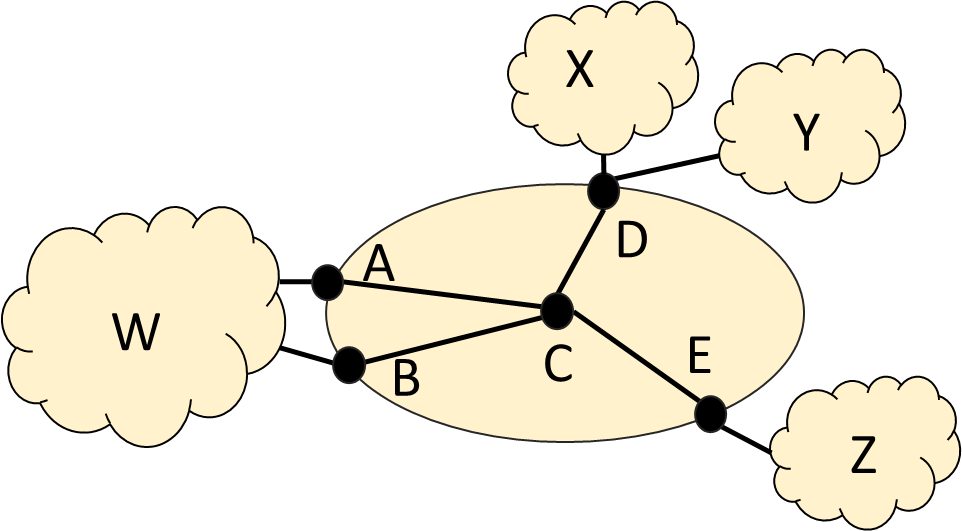
\includegraphics[width=.8\columnwidth]{figures/topology}

  \hdr{\large Policy Automata}{}
  \vspace*{1\baselineskip}

  \begin{tikzpicture}[>=stealth',shorten >=1pt,auto,node distance=1.6cm]
    \state{0}{$0$}{              }{}
    \state{1}{$1$}{right of=0}{}
    \state{2}{$2$}{right of=1}{}
    \state{3}{$3$}{right of=2}{}
    \state{4}{$4$}{right of=3}{}
    \state{5}{$5$}{right of=4}{accepting}
    \transition{0}{1}{out}{}
    \transition{1}{2}{D}{}
    \transition{2}{3}{C}{}
    \transition{3}{4}{A}{}
    \transition{4}{5}{W}{}
  \end{tikzpicture}

  \begin{tikzpicture}[>=stealth',shorten >=1pt,auto,node distance=1.6cm]
    \state{0}{$0$}{              }{}
    \state{1}{$1$}{right of=0}{}
    \state{2}{$2$}{right of=1}{}
    \state{3}{$3$}{right of=2}{}
    \state{4}{$4$}{right of=3}{accepting}
    \transition{0}{1}{out}{}
    \transition{1}{2}{in}{}
    \transition{2}{2}{A,C,D,E}{loop above}
    \transition{2}{3}{B}{}
    \transition{3}{3}{B}{loop above}
    \transition{3}{2}{A,C,D,E}{bend left}
    \transition{3}{4}{W}{}
  \end{tikzpicture}


  \end{minipage}
  %
  ~~
  ~~
  %
  \begin{minipage}[t]{.5\linewidth}
  \hdr{\large Product Graph}{}
  \vspace*{-1\baselineskip}
  %
  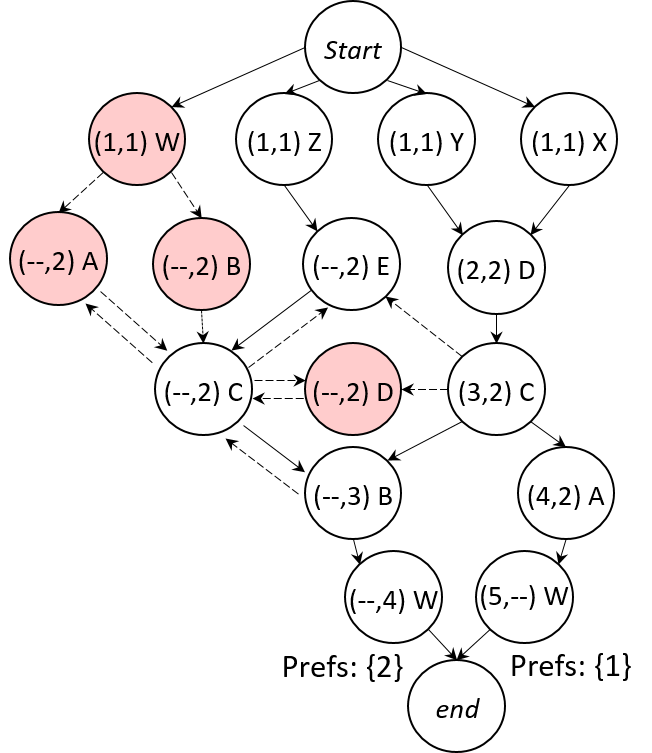
\includegraphics[width=.8\columnwidth]{figures/productgraph}
  \end{minipage}

  \hrulefill

  \caption{Example Product graph construction.}
  \label{fig:example-compilation}
\end{figure*}


Now that the user policy exists in a simplified form, we must take the topology into consideration. In particular, we are interested in a compact representation that describes all the possible ways BGP route advertisements can flow through the network subject to the policy and topology constraints. To this end, we use a Product Graph Intermediate Representation (PGIR) to capture these dependencies. The Product graph can be thought of as the intersection of each of the regular automata corresponding to the RIR path preferences, and the topology. Paths through the product graph will correspond to real paths through the topology that satisfy the user constraints. Finding paths through a graph subject to regular constraints has been studied extensively in the database literature~\ref{bib:todo}, and has been applied to networks in the past~\ref{bib:todo}.

\para{Formal definition}

% Formally define automata
The translated user policy into RIR is of the form $r_1 \gg \dots \gg r_j$. While paths talk about the direction traffic flows through the network, to implement the policy with BGP we are concerned about the way control-plane information is disseminated (i.e., router advertisements flowing in the opposite direction). To capture this idea, for each regular expression $r_i$, we construct a deterministic finite state machine on the reversed regular expression. Each automaton is a tuple: ($\Sigma, Q_i, F_i, q_{0_i}, \sigma_i$). The alphabet $\Sigma$ consists of all internal and external ASes, $Q_i$ is the set of states for automaton i, $F_i$ is the set of final states, $q_{0_i}$ is the initial state, and $\sigma_i \colon Q_i \times \Sigma \rightarrow Q_i$ is the state transition function.
%
% Formally define topology
The topology is represented as a graph ($V, E$), which consists of a set of vertices $V$, and a set of directed edges $E \colon 2^{V \times V}$.
%
% Formally define product graph
The combined product graph is a tuple: ($V'$, $E'$, $s$, $e$, $P$) with
vertices $V' \colon V \times Q_1 \times \dots \times Q_j$,
edges $E' \colon 2^{V' \times V'}$,
a unique starting vertex $s$,
a unique ending vertex $e$,
and a preference function $P \colon V \rightarrow 2^{\set{1, \dots, j}}$ , which maps nodes in the product graph to a set of preference ranks.
For a vertex $v' = (v, \dots) \in V'$, we say $loc(v') = v$. We say a node $x$ shadows node $y$ in the product graph when $x \in V'$ and $y \in V'$ and $loc(x) = loc(y)$ but $x \neq y$. That is, $x$ shadows $y$ when they are different nodes in the PGIR that represent the same topology location.

\para{From RIR To PGIR}

% Formal product construction
Let $a_i$ and $b_i$ stand for states in the regular policy automata.
The product graph is constructed by adding an edge from $v_1 = (x, a_1, \dots, a_m)$ to $v_2 = (y, b_1, \dots, b_m)$ whenever $\sigma_i(a_i, y) = b_i$ for each $i$ and $(x,y) \in E$ is a valid topology link.
%
Additionally, we add edges from the start node $s$ to any $v = (x, a_1, \dots, a_m)$ when $\sigma_i(q_{0_i}, x) = a_i$ for each $i$.
%
The preference function $P$ for node $v = (x, a_1, \dots, a_m)$ is defined as $P(v) = \set{i~\vert~a_i \in F_i} $. That is, it records which preferences are achieved for the policy automata for each node in the product construction.
%
Finally, there is an edge from each node in the product graph such that $P(v) \neq \emptyset$ to the special end node $e$.


Intuitively the product graph tracks which states of each automaton the policy is in as route advertisements move between routers in the topology.
%
Consider the topology shown in Figure~\ref{fig:example-compilation}. Suppose we want to set up a primary route from W that enters the network from $A$, and utilizes the A -- C and C -- D links. We also would like a backup route that enters from node $B$, and utilizes the B -- C link, but is otherwise unconstrained. For the sake of simplicity, we will assume that the route can end in either $X$, $Y$, or $Z$. The RIR for the policy is:
%
$$(W \cdot A \cdot C \cdot D \cdot out) \gg (W \cdot B \cdot in^* \cdot out)$$
%
Figure~\ref{fig:example-compilation} shows the policy automata for each regular expression preference. Since we are interested in the flow of control messages, the automata match backwards.
%
Figure~\ref{fig:example-compilation} shows the product graph obtained from intersecting the topology and policy automata. Every path in the product graph corresponds to a concrete path in the topology. In particular, every path through the product graph that ends at a node $v$ such that the preference function $P(v) = \set{i_1, \dots, i_m}$ is non-empty, is a valid topological path that satisfies the policy constraints and results in a particular path with preferences $i_1$ through $i_m$.
%
For example, the path $X \cdot D \cdot C \cdot A \cdot W$ is a valid path in the topology that BGP route advertisements might take, which would lead to obtaining the most prefered preference $1$.
BGP control messages can start from peer X, which would match the $out$ transition from both automata, leading to state $1$ in the first automaton, and state $1$ in the second automaton. This is reflected in the product graph by the node with state $(1,1) X$. From here, if X were to advertise this route to D, it would result in the path $D X$, which would lead to state $2$ in the first automaton, and state $2$ in the second automaton, and so on. The $-$ state indicates it is dropped from the corresponding automaton. Since node $(5,-) W$ is in an accepting state for the first automata, it indicates this path has preference 1.

\para{Minimization}

Although every path through the product graph is a valid path in the topology, we do not want to consider loops when configuring the network. In particular, BGP's loop prevention mechanism (where an AS rejects any route for which it is already in the AS path), means that loops should never occur.\footnote{Note: misconfigured aggregation can still lead to loops in BGP}
%
However, the product graph may contain many paths that form loops in the topology. For example, in Figure~\ref{fig:example-compilation}, the path $W \cdot A \cdot C \cdot B \cdot W$ is a valid path that BGP route advertisements might take through the topology, leading to a path that satisfies the preference 1 policy, but which contains a loop.
%
Since we are primarily concerned with guaranteeing user policy correctness and safety with respect to network failures, it is useful to avoid considering cases that are not possible due to loops. For example, if we can safely remove an edge from the product graph, then we don't have to consider what happens when the edge has failed.

We can safely remove any node or edge from the product graph so long as it never appears on any \emph{simple} path from the \textit{start} node to the \emph{end} node. For example, node $(1,1) W$ in Figure~\ref{fig:example-compilation} is never on a simple path to the end node since it most go through another $W$ in either case.
%
Although fully minimizing the product graph is an NP-complete problem, we find that a simple and efficient algorithm based on graph dominators achieves largely the same effect, greatly simplifying the failure safety analysis.

A node $x$ dominates node $y$ if $x$ appears on every path leading to $y$ from a source node. Many algorithms for finding graph dominators efficiently exist~\ref{bib:todo}. For minimization, we compute the dominator set for each node in both the product graph $G$ with respect to the start node, and in the reversed product graph $G^R$ with respect to the end node. The following rules enable efficient minimization of the product graph.
%
\begin{itemize}
  \item Remove nodes that never reach the end node
  \item Remove nodes not reachable from the $start$ node
  \item Remove any node $x$ such that $x$ is dominated by $y$ in $G$ or $G^R$, and $loc(x) = loc(y)$
  \item Remove any edge from $x$ to $y$ in $G$ or $G^R$ if there is some node $z$ dominated by $y$ such that $loc(x) = loc(z)$
\end{itemize}
%
Repeated application of the above rules leads to removing the colored nodes and dashed lines in Figure~\ref{fig:example-compilation}.

\para{Failure Safety}

To implement path preferences in routing, BGP uses local preferences on a per-device basis. However, the distributed nature of BGP makes setting preferences locally to achieve a network-route routing policy difficult, particularly in the presence of failures. For example, imagine an extremely simple policy for the topology in Figure~\ref{fig:example-compilation}, which says to prefer one route over another:
%
$$(W \cdot A \cdot C \cdot D) \gg (W \cdot B \cdot C \cdot E)$$
%
How could such a policy be implemented in BGP? Suppose we simply set the local preference at router $C$ to prefer $D$ over $E$. However, now if the A -- C link fails, then suddenly $C$ has made the wrong decision and can not get either the primary or backup route specified, despite the fact that the $W \cdot B \cdot C \cdot E$ path is available.

At a first cut, any time a router must make a decision locally between several route options, there is the possibility that it might choose incorrectly. The product graph representation captures this notion of choice precisely. For example, router $D$ in Figure~\ref{fig:example-compilation} appears only once in the product graph, possibly receiving route advertisements from $X$ or $Y$. However, regardless of whether $D$ chooses a route from $X$ or $Y$, the set of paths allowed by the policy after going through $D$ will be the same in either case. This remains true despite any failures that might have occurred in the network. Thus $D$ can safely prefer $X$ and $Y$ equally.

The more challenging case is when a topology location occurs in mutliple contexts in the product graph. For example, in the compilation example from Figure~\ref{fig:example-compilation}, the topology node $C$ can receive an advertisement from $E$ and later achieve the backup path, or it can receive an advertisement from its neighbor $D$ and later achieve either the primary or backup path. Is it safe for $C$ to prefer its neighbor $D$ over its other neighbor $E$? The important observation is that, if $C$ prefers $D$, then it is never worse off -- it will always achieve at least as good a path as if it had choosen $E$.
For example, suppose $C$ chooses a route from $D$, but cannot achieve its primary path because the $A$ -- $W$ link has failed. In this case, the advertisement from $C$ will still be sent along towards the ultimate backup location $W$. Since the $(3,2) C$ node has the same one-step and two-step next hops as node $(-,2) C$ in the product graph, no possible failure will prevent a route advertisment from reaching $(-,4) W$ that wouldn't have otherwise prevented it if $C$ had choosen $E$.

In general, ensuring that an individual router's preferences respect the policy under all possible failures is hard, and a simple enumeration of failures is intractable. Instead, we adopt a conservative analysis based on the product graph representation and the previous observations. The high-level idea is to order each node in the product graph according to a \textit{can prefer} relation. For example, node $(3,2) C$ can be preferred to node $(-,2) C$, but not the other way around. Intuitively, a node $N_1$ can be preferred to another node $N_2$ when, for each preference $N_2$ might achieve, there is a better preference that $N_1$ will achieve regardless of failures. Formally this means that $N_1$ can be preferred to $N_2$ when:
%
$$\forall i, \exists j, j \leq i \wedge protect(G_j, N_1, G_i, N_2)$$
%
where the \textit{protect} predicate means that, from $N_1$ on the product graph restricted nodes that can potentially achieve preference $j$ or better, there are at least as many paths as from $N_2$ restricted to $G_i$

\begin{algorithm}[t!]
\caption{Failure Protection}
\label{alg:failures}
\begin{algorithmic}[1]
\Procedure{Protect($G_1$, $N_1$, $G_2$, $N_2$)}{}
  \If {$loc(N_1) \neq loc(N_2)$} \Return false
  \EndIf
  \State $q \gets Queue()$
  \State $q.Enqueue (N_1, N_2)$
  \While {$!q.Empty()$}
    \State $(n_1,n_2) \gets q.Dequeue()$
    \For {$x$ in $adj(G_2, n_2)$}
      \If {some $y$ in $adj(G_1,n_1)$ shadows $x$}
        \If {$(x,y)$ not marked}
          \State {mark $(x,y)$ as seen}
          \State $q.Enqueue(x,y)$
        \EndIf
      \Else { \Return $false$}
      \EndIf
    \EndFor
  \EndWhile
  \Return true
  \EndProcedure
\end{algorithmic}
\end{algorithm}

The algorithm listed in Algorithm~\ref{alg:failures} defines what it means for one node to \textit{protect} against the failures of another. The algorithm walks from nodes $N_1$ and $N_2$ in $G_j$ and $G_i$ respectively, and ensures that for every \textit{step} $N_2$ can take to some new topology location, $N_1$ can, at the very least, take an equivalent step. Thus any paths leading from $N_2$ will have an equivalent path over the same topology locations from $N_1$. Algorithm~\ref{alg:failures} works because each node in the product graph can have at most one outgoing neighbor with the same topological location, so the next hop neighbors can be checked without backtracking. The algorithm terminates since the number of related states $(x,y)$ that can be expolored is finite.
\ryan{Add the new part that goes up to a dominating predecessor when no other option}

Local preferences are now obtained by, for each router in the topology, sorting the corresponding nodes in the product graph according to \textit{can prefer} relation. If two nodes are incomparable, then the compiler rejects the policy as unimplementable.
\ryan{We are checking if the preorder forms a partial order by satisfying asymmetry}

\para{Avoiding Simple Paths}

The checks for failure safety described previously overlook one critical point: even if the analysis determines that a node $x$ protects against failures of another node $y$, it may be tricked into thinking $x$ has a particular path that will actually be discarded by BGP's loop prevention mechanism due to locations previously traversed before arriving at $x$. To avoid this situation, the compiler conservatively checks that $x$ protects against $y$ without using any nodes that shadow another node that appears above $x$ in the product graph (i.e., nodes reachable from $x$ in $G_j^R$). It is fine however, to reuse the same nodes that appear above $x$, since any path that went through another node $z$ to get to $x$, but then looped through $z$ again, would be obtainable from $z$ itself.
\ryan{rework this}


\subsection{Abstract BGP}

%\begin{figure}[t!]
%\centering
%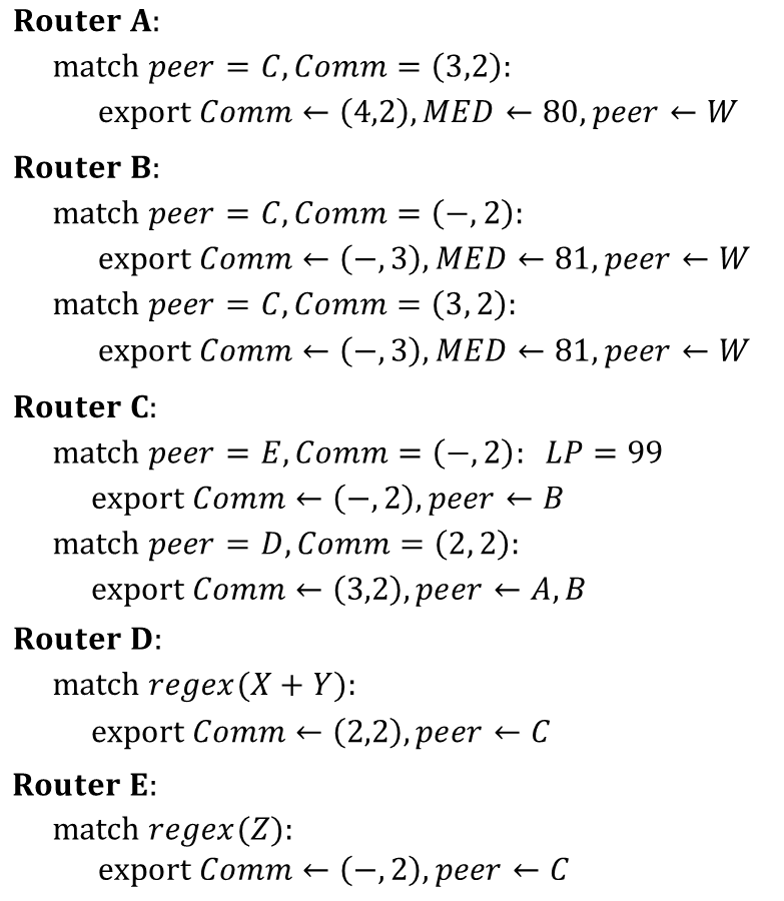
\includegraphics[width=.9\columnwidth]{figures/config}
%\caption{Abstract BGP configuration.}
%\label{fig:abgp-config}
%\end{figure}

\newcommand{\highlight}[1]{%
  \colorbox{red!50}{$\displaystyle#1$}}
\newcommand{\Router}[1]{ \textbf{Router #1:} }
\newcommand{\REGEX}[1]{ \text{regex}(#1) }
\newcommand{\PEER}{ \text{peer} }
\newcommand{\COMM} {\text{comm}}
\newcommand{\MED} {\text{MED}}

\begin{figure}[t!]
\begin{lstlisting}[frame=single, mathescape=true]
$\Router{A}$
  Match $\PEER=C, \COMM=(3,2)$
    Export $\COMM \leftarrow (4,2), \MED \leftarrow 80, \PEER \leftarrow W$
$\Router{B}$
  Match $\PEER = C, \COMM = (-,2)$
    Export $\COMM \leftarrow (-,3), \COMM \leftarrow \text{noexport},$
           $\MED \leftarrow 81, \PEER \leftarrow W$
  Match $\PEER = C, \COMM = (3,2)$
    Export $\COMM \leftarrow (-,3), \COMM \leftarrow \text{noexport},$
           $\MED \leftarrow 81, \PEER \leftarrow W$
$\Router{C}$-
  Match$[LP=99]$ $\PEER = E, \COMM = (-,2) $
    Export $\COMM \leftarrow (-,2), \PEER \leftarrow B$
  Match $\PEER = D, \COMM = (2,2)$
    Export $\COMM \leftarrow (3,2), \PEER \leftarrow A,B$
$\Router{D}$
  Match $\REGEX{X + Y}$
    Export $\COMM \leftarrow (2,2), \PEER \leftarrow C$
$\Router{E}$
  Match $\REGEX{Z}$
    Export $\COMM \leftarrow (-,2), \PEER \leftarrow C$
\end{lstlisting}
\label{fig:config}
\caption{Abstract BGP router configurations.}
\end{figure}


%\begin{figure}[t!]
%\begin{lstlisting}[frame=single, mathescape=true]
%$\Router{A}$
%  Match $\PEER=C$
%    Export $\MED \leftarrow 80, \PEER \leftarrow W$
%$\Router{B}$
%  Match $\PEER = C$
%    Export $\COMM \leftarrow \text{noexport}, \MED \leftarrow 81, \PEER \leftarrow W$
%$\Router{C}$
%  Match$[LP=99]$ $\PEER = E $
%    Export $\PEER \leftarrow B$
%  Match $\PEER = D$
%    Export $\PEER \leftarrow A,B$
%$\Router{D}$
%  Match $\REGEX{X + Y}$
%    Export $\PEER \leftarrow C$
%$\Router{E}$
%  Match $\REGEX{Z}$
%    Export $\PEER \leftarrow C$
%\end{lstlisting}
%\label{fig:config-min}
%\caption{Abstract BGP minimized configurations}
%\end{figure}

The final stages of compilation consist in translating policies from PGIR to a simple, vendor-neutral abstraction of BGP (ABGP), and then translating from ABGP to actual device configurations.

\para{From PGIR to ABGP}

Having found a total ordering on node preferences in the product graph from the failure safety analysis, the translation to ABGP becomes straightforward. The idea is to encode the state of the automaton using BGP community values. Each router will match based on its peer and a community value corresponding to the state of the product graph, and then update the state before exporting to the neighbors permitted according to the product graph. For example, router $A$ from the example in Figure~\ref{fig:example-compilation} will allow an advertisement from its peer $C$ with a community value for state $(3,2)$ (and deny anything else). If it sees such an advertisement, it will remove the old community value, and add a new community value for state $(4,2)$ before exporting the route to its neighbor $W$.

To ensure preferred paths are always obtained, for each router $r$ in the topology, the compiler will simply set a higher local preference for neighbors of a more-preferred node for $r$ in the product graph. For example, $C$ will prefer an advertisement from $D$ in state $(2,2)$ over an advertisement from $E$ in state $(-,2)$.

Since the compiler is only able to control community tagging only for routers under the control of the AS being programmed, it cannot match on communities for external ASes. Instead, it simply translates matches from external ASes into a BGP regular expression filter. For example, node $D$ in Figure~\ref{fig:example-compilation} would match the single hop external paths $X$ or $Y$ and prefer them equally. In general, if routes are allowed from beyond $X$ or $Y$, these will also be captured in the BGP regular expression filters. In practice, we model the unknown AS topology as a special node in the product graph that generates a filter to match any sequence of ASes.

Finally, in our example, the external AS $W$ would need to prefer our internal router $A$ over $B$. In general, it is not possible to control traffic entering the network beyond certain special cases. In this example however, the BGP MED attribute can influence $W$ to prefer $A$ over $B$ since the preference is for a single external peer.  Additionally, the compiler can use the BGP no-export community can ensure that no other AS beyond $W$ can send us traffic. The compiler can perform a simple analysis to determine when it can utilize various BGP special attributes to ensure traffic enters the network in a particular way by looking at links in the product graph that cross from the internal topology to the external topology. Aggregation is another tool commonly used to influence how traffic can enter the network, by relying on BGP's longest prefix matching default. Since aggregates are provided as additional user constraints, the compiler can also make use of this information to check that incoming preferences can be met given the aggregates specified (e.g., to ensure that all external ASes prefer to enter from one location over another).

Figure~\ref{fig:config} shows the full configuration from the compilation example. To make configurations more compact and readable, the \sysname compiler will rewrite configurations in ABGP - for example removing community tagging and matching when there is no ambiguity. Figure~\ref{config-min} shows the minimized router configurations.



\subsection{Aggregation-Induced Black Holes}

\begin{figure}[t!]
\centering
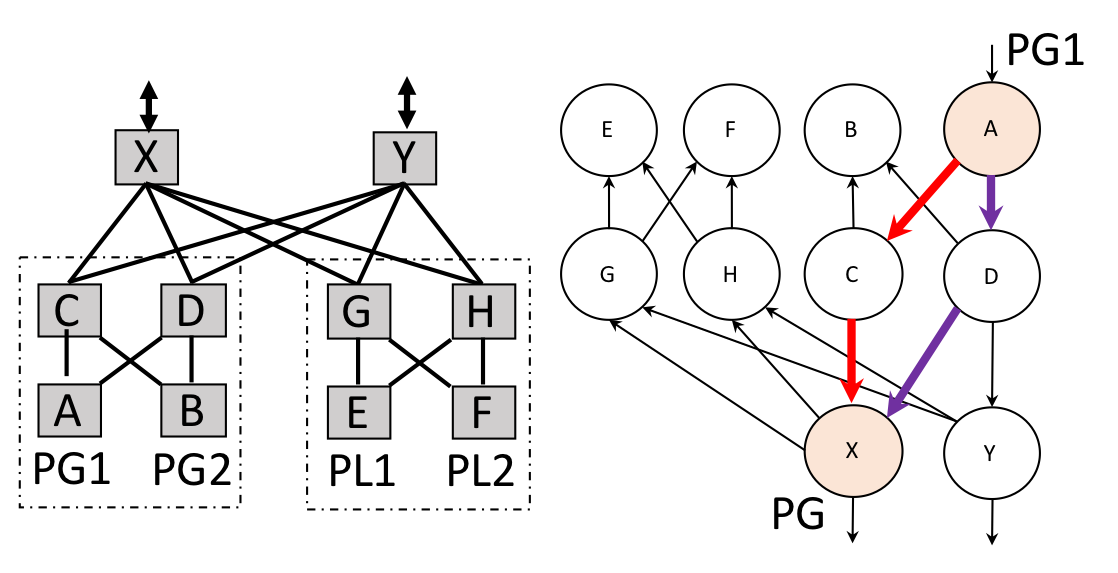
\includegraphics[width=\columnwidth]{figures/aggregation}
\caption{Aggregation safety.}
\label{fig:aggregation-safety}
\end{figure}

As was demonstrated in Example 2 of Section~\ref{sec:motivation}, the use of aggregation in BGP can lead to subtle black-holing traffic when failures occur. Deciding when this can happen requires knowledge of the routing policy and not just the topology. For instance, a policy might require all traffic for a particular prefix going through a router where an aggregate is advertised to go over a single link, even if there are several available in the toplogy. If the single link fails, then a black hole might be introduced. Fortunately, the PGIR captures this information precisely, describing the how information meeting the policy flows over the topology.

We can frame the aggregation problem as a problem of connectivity in the PGIR. More specifically, for each prefix that falls under an aggregate, we find a lower bound on the number of failures that would disconnect where the prefix originates from where its more specific aggregate is located. The difficulty lies in the fact that the same links in the topology can appear in multiple places in the PGIR. We adopt the following simple strategy to lower bound the number of failures:
\begin{enumerate}
	\item Pick a random path through the product graph from start to end.
	\item Remove all edges in the product graph corresponding to the set of topological edges choosen.
	\item Repeat until no path exists.
\end{enumerate}
Since each path through the PGIR will result in a new edge-disjoint path through the topology (since we have removed all already used edges), and since the number of edge-disjoint paths through the topology is no more than the min-cut. \todo{clarify this}

For example, imagine we use the earlier data center example from Section~\ref{sec:motivation}, with the policy: $p_{g1} \mapsto end(A)$, where $p_{g1}$ falls under the $p_{g^*}$ aggregate. The data center topology and a simplification of the corresponding product graph are shown in Figure~\ref{fig:aggregation-safety}. Since the compiler knows an aggregate will be placed at $X$, and it knows that, for prefix $p_{g1}$ the route will originate at $A$, we can compute the number of failures it would take to disconnect $A$ from $X$ in the product graph. In this case, we could remove the $A$ -- $D$ -- $X$ path first. We would then need to remove any other $A$ -- $D$ or $D$ -- $X$ links from the product graph, though in this case there are none. Next, we could remove the links along the $A$ -- $C$ -- $X$ path, repeating the process. Because afterwards $A$ is disconnected from $X$, the compiler knowns that 2 is a lower bound on the number of failures for aggregation safety for prefix $p_{g1}$. This process is then repeated for other aggregation locations (e.g., $Y$).


